% !TEX root = epifanov_solid_state_physics.tex
%!TEX TS-program = pdflatex
%!TEX encoding = UTF-8 Unicode


\chapter[Thermoelectric and Galvanomagnetic
Phenomena]{Thermoelectric and Galvanomagnetic\\
Phenomena}\label{chap:9}
\chaptermark{Thermoelectric and Galvanomagnetic
Phenomena}

% \noindent
The thermoelectric effects include the Seebeck, the Peltier, and the Thomson effects, and the galvanomagnetic the Hall, the Ettingshausen, and the Nernst effects. Some of those phenomena have found wide application in practice; therefore, a look at them is not only of educational but of practical interest as well.

Let us discuss briefly the physical background of those phenomena.

\section{The Seebeck effect}\label{sec:79}

In 1822, T. J. Seebeck discovered that an electromotive force $\ab{V}{T}$ is established in a circuit consisting of two conductors $1$ and $2$ made of different materials if the junctions of these conductors, A and B, are kept at different temperatures, $T_1$ and $T_2$ [\fig{9_1}(a)]. This emf is termed \textit{thermal emf}. Experiments show it to be---in a narrow temperature interval---proportional to the difference in the temperature of the junctions A and B:
\begin{equation}\label{eq:9_1}
    \ab{V}{T} = \alpha (T_2 - T_1).
\end{equation}

The proportionality factor
\begin{equation}\label{eq:9_2}
    \alpha = \diff{\ab{V}{T}}{T}
\end{equation}

\noindent
is called \textit{differential}, or \textit{specific}, \textit{thermoelectric power}. It is determined by the material of the conductors and the temperature.

There are three sources of thermal emf: the directional current of the carriers in the conductor due to the presence of a temperature gradient (the volumetric component $\ab{V}{V}$), the change in the position of the Fermi level (the junction component $\ab{V}{j}$), and the drag of the electrons by the phonons (the so-called phonon drag effect).

Let us discuss the physical nature of each of those sources.

\textbf{Volumetric component of thermal emf.} Suppose that a temperature difference $(T_2 - T_1)$ is maintained at the terminals of a uniform conductor AB [\fig{9_1}(b)], so that there is a temperature gradient $\diffin{T}{x}$ in the direction from B to A. The current carriers in the hot end have greater kinetic energy and greater speeds of motion than the carriers in the cold end. Therefore, a current will flow in the conductor from the hot end to the cold; this current will charge the conductor. In cases when the current is carried by electrons, the cold end will accumulate a negative charge and the hot end a positive charge, and a potential difference $\ab{V}{V}$ will be established between them. This is the volumetric component of thermal emf. The differential thermoelectric power corresponding to this component is
\begin{equation}\label{eq:9_3}
    \ab{\alpha}{V} = \diffpartial{\ab{V}{V}}{T},
\end{equation}

\noindent
$\ab{\alpha}{V}$ may be estimated as follows. The pressure of the electron gas in the conductor is
\begin{equation}\label{eq:9_4}
    p = \frac{2}{3} n \overline{E},
\end{equation}

\noindent
where $\overline{E}$ is the average energy of electrons in the conductor, and $n$ their concentration.

\begin{figure}[t]
	\begin{center}
		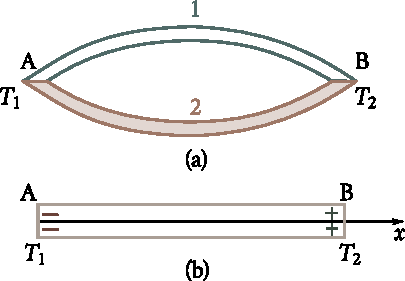
\includegraphics[scale=0.9]{figures/ch_09/fig_9_1.pdf}
		\caption[]{The Seebeck effect: (a)---thermoelectric circuit; (b)---origin of volumetric and junction components of thermal emf.}
		\label{fig:9_1}
	\end{center}
	\vspace{-0.9cm}
\end{figure}

The temperature gradient occasions a pressure gradient to compensate which a field $\mathcal{E}$ should be established in the conductor such that
\begin{equation*}
    q \mathcal{E} n = \diffpartial{p}{x} = \diffpartial{p}{T} \diffpartial{T}{x}.
\end{equation*}

\noindent
From here, $\ab{\alpha}{V}$ may easily be found:
\begin{equation}\label{eq:9_5}
    \ab{\alpha}{V} = \diffpartial{\ab{V}{V}}{T} = \mathcal{E} \parenthesis{\diffpartial{T}{x}}^{-1} = \frac{1}{nq} \diffpartial{p}{T}.
\end{equation}

As a rule, in an n-type conductor, $\ab{\alpha}{V}$ is directed from the hot end to the cold. However, there are exceptions to this rule which we will discuss below.

\textbf{The junction component of thermal emf.} The change in temperature occasions a change in the position of the Fermi level. In n-type conductors, the Fermi level sinks on the energy diagram as the temperature is raised [see \fig{5_19}(a)]. By force of this it should be higher on the cold end of an n-type conductor than on its hot end. The difference in the Fermi level positions is equivalent to a potential difference
\begin{equation}\label{eq:9_6}
    \deriv{\ab{V}{j}} = -\frac{1}{q} \diffpartial{\mu}{T}\, \deriv{T}.
\end{equation}

\noindent
And this is just the \textit{junction component} of the thermal emf. The differential thermoelectric power corresponding to this component is
\begin{equation}\label{eq:9_7}
    \ab{\alpha}{j} = -\frac{1}{q} \diffpartial{\mu}{T}.
\end{equation}

The resultant differential thermoelectric power
\begin{equation}\label{eq:9_8}
    \alpha = \frac{1}{nq} \diffpartial{p}{T} - \frac{1}{q} \diffpartial{\mu}{T}.
\end{equation}

\noindent
We apply the relation \eqref{eq:9_8} to conductors of various kinds.

\textbf{Thermoelectric power of metals.} Substituting the average energy of electrons of a degenerate electron gas from \eqn{3_45} into \eqref{eq:9_4}, we obtain the following expression for the pressure of the electron gas in a metal:
\begin{equation*}
    p = \frac{2}{3} n \overline{E} =\frac{2}{5} n \ab{E}{F} + \frac{\pi^2}{6\ab{E}{F}} (\ab{k}{B}T)^2.
\end{equation*}

\noindent
Differentiating this expression with respect to $T$ and multiplying it by $1/nq$, we obtain
\begin{equation}\label{eq:9_9}
    \ab{\alpha}{V} = \frac{\ab{k}{B}}{q} \frac{\pi^2}{3} \frac{\ab{k}{B}T}{\ab{E}{F}}.
\end{equation}

The temperature dependence of the Fermi level in metals is given by relation \eqref{eq:3_44}:
\begin{equation*}
    \mu = \ab{E}{F} \bracket{1 - \frac{\pi^2}{12} \parenthesis{\frac{\ab{k}{B}T}{\ab{E}{F}}}^2}.
\end{equation*}

\noindent
Differentiating it with respect to $T$ and multiplying by $1/q$, we obtain
\begin{equation}\label{eq:9_10}
    \ab{\alpha}{j} = - \frac{\pi^2 \ab{k}{B}}{6q} \frac{\ab{k}{B}T}{\ab{E}{F}}.
\end{equation}

\noindent
Substituting \eqns{9_9}{9_10} into \eqref{eq:9_8}, we obtain
\begin{equation}\label{eq:9_11}
    \ab{\alpha}{m} = \frac{\pi^2 \ab{k}{B}}{3q} \parenthesis{1 + \frac{1}{2}} \frac{\ab{k}{B}T}{\ab{E}{F}}.
\end{equation}

A more accurate calculation for metals with a quadratic dependence of the electron energy on the wave vector produces the following result:
\begin{equation}\label{eq:9_12}
    \ab{\alpha}{m} = \frac{\pi^2 \ab{k}{B}}{3q} \parenthesis{1+r} \frac{\ab{k}{B}T}{\ab{E}{F}},
\end{equation}

\noindent
where $r$ is the exponent in the relation
\begin{equation}\label{eq:9_13}
    \lambda \propto E^r,
\end{equation}

\noindent
which expresses the dependence of the electron mean free path on energy $E$.

Table \ref{table:9_1} presents the values of $r$ for various mechanisms of electron scattering on atomic-and ionic lattices.

\begin{table}[!b]
	\renewcommand{\arraystretch}{1.2}
	\caption{}
	\vspace{-0.6cm}
	\label{table:9_1}
	\begin{center}\resizebox{0.98\linewidth}{!}{
			\begin{tabular}{lcccc}
				\toprule[1pt]
                 & \multicolumn{3}{c}{\textbf{Scattering on thermal vibrations}} & \multirow{3}{*}{\textbf{Scattering on impurity atoms}}\\
                 \cline{2-4}
                 & \multirow{2}{*}{\textbf{Atomic lattice}} & \multicolumn{2}{c}{\textbf{Ionic lattice}} & \\
                 \cline{3-4}
                 & & $T<\theta$ & $T>\theta$ & \\
                \midrule[0.5pt]\midrule[0.5pt]
                $r$ & $0$ & $1/2$ & $1$ & $2$\\
				\bottomrule[1pt]
			\end{tabular}
	}\end{center}
\end{table}

It follows from \eqn{9_12} that for metals $\ab{\alpha}{m}\propto T$, in full agreement with experiment. Since $\ab{k}{B}T\ll\ab{E}{F}$, the thermoelectric power of metals is quite small. For instance, for silver $\ab{E}{F}=\SI{5.5}{\electronvolt}$ and $\ab{k}{B}T=\SI{0.025}{\electronvolt}$ at $T=\SI{300}{\kelvin}$.
Substituting this into \eqn{9_12}, we obtain $\ab{\alpha}{m}\approx\SI{8e-6}{\volt\per\kelvin}$, which is quite close to the experimental value $\ab{\alpha}{m}\approx\SI{5e-6}{\volt\per\kelvin}$.

It follows from \eqn{9_13}, that when $r<0$ the more energetic electrons have a shorter mean free path $\lambda$. Since the diffusion current in this case is directed from the hot end to the cold end, the sign of the volumetric component of the thermal emf will be reversed. This may cause the reversal of the sign of the metal's thermal emf as a whole. Such effects are observed, for example, in some transition metals and in some alloys.

As was already stated before, \eqn{9_12} is valid for metals with a quadratic $E(k)$ dependence. In metals and in alloys with a complex Fermi surface, the contribution of the various regions of this surface may differ not only in absolute value but in sign as well, with the result that the thermoelectric power may be zero or close to zero. For instance, lead has a zero thermoelectric power. For this reason, thermoelectric power is usually measured in relation to lead.

The current direction in the hot junction of a thermocouple made of an n-type conductor and of lead will be determined by the polarity of the conductor's charge. For a normal conductor whose hot junction acquires a positive charge, the current in it will be directed from conductor to lead [\fig{9_2}(a)]. In this case, the conductor's thermoelectric power is assumed to be negative.

\begin{figure}[t]
	\begin{center}
		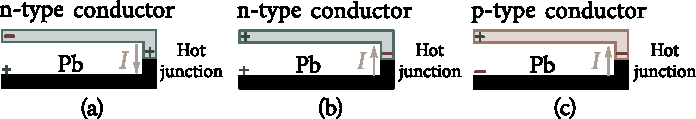
\includegraphics[scale=1]{figures/ch_09/fig_9_2.pdf}
		\caption[]{Magnitude and sign of thermoelectric power determined in relation to lead (explanation in text).}
		\label{fig:9_2}
	\end{center}
	\vspace{-0.9cm}
\end{figure}

In case of an n-type conductor acquiring an anomalous charge [\fig{9_2}(b)], the current in the hot junction will flow from lead to conductor and a will be positive; $\lambda$ will be positive for a normal p-type conductor too, whose hot end acquires a negative charge [\fig{9_2}(c)].

\textbf{Thermoelectric power of semiconductors.} The pressure of electron gas in a nondegenerate semiconductor is
\begin{equation*}
    p = \frac{2}{3} n \overline{E} = n \ab{k}{B}T.
\end{equation*}

\noindent
Differentiating this expression with respect to $T$ and multiplying by $1/nq$, we obtain
\begin{equation}\label{eq:9_14}
    \ab{\alpha}{V} = \frac{\ab{k}{B}}{q} \bracket{1 + T \diffpartial{\ln{n}}{T}}.
\end{equation}

\noindent
A more rigorous calculation yields
\begin{equation}\label{eq:9_15}
    \ab{\alpha}{V} = \frac{\ab{k}{B}}{q} \bracket{r + \frac{1}{2} + T \diffpartial{\ln{n}}{T}}.
\end{equation}

\noindent
The chemical potential in a nondegenerate n-type semiconductor is given by relation \eqref{eq:3_26}:
\begin{equation*}
    \ab{\mu}{n} = \ab{k}{B} T \ln\bracket{\frac{nh^3}{2(2\pi\ab{m}{n}\ab{k}{B}T)^{3/2}}}.
\end{equation*}

\noindent
Differentiating $\ab{\mu}{n}$ with respect to $T$ and multiplying by $1/q$, we obtain
\begin{equation}\label{eq:9_16}
    \ab{\alpha}{j} = \frac{\ab{k}{B}}{q} \parenthesis{ \frac{3}{2} - \frac{\ab{\mu}{n}}{\ab{k}{B}T} - T \diffpartial{\ln{n}}{T}}.
\end{equation}

\noindent
Substituting \eqns{9_15}{9_16} into \eqref{eq:9_8}, we obtain
\begin{equation}\label{eq:9_17}
    \ab{\alpha}{n} = - \frac{\ab{k}{B}}{q} \parenthesis{r + 2 - \frac{\ab{\mu}{n}}{\ab{k}{B}T}} = - \frac{\ab{k}{B}}{q} \bracet{r + 2 + \ln\bracket{\frac{2(2\pi\ab{m}{n}\ab{k}{B}T)^{3/2}}{nh^3}}}.
\end{equation}

\noindent
The minus sign in front of the right-hand side is in accordance with the conventional polarity of the thermoelectric power.

For a n-type semiconductor
\begin{equation}\label{eq:9_18}
    \ab{\alpha}{p} = \frac{\ab{k}{B}}{q} \bracet{r + 2 + \ln\bracket{\frac{2 (2 \pi \ab{m}{p} \ab{k}{B} T)^{3/2}}{ph^3}}}.
\end{equation}

Let us estimate the value of $\alpha$ of an extrinsic semiconductor, for instance, for n-type germanium with $n=\SI{e23}{\per\metre\cubed}$ at $T=\SI{300}{\kelvin}$. Substituting those values into \eqn{9_17}, we obtain $\alpha\approx\SI{e-3}{\volt\per\kelvin}$. Hence, the thermoelectric power of semiconductors is three orders of magnitude greater than that of metals.

For semiconductors with bipolar conductivity, in which the electric current is carried both by electrons and holes, the expression for the thermoelectric power is:
\begin{equation}\label{eq:9_19}
    \ab{\alpha}{n,p} = \frac{\ab{\alpha}{p} p \ab{u}{p} - \ab{\alpha}{n} n \ab{u}{n}}{p \ab{u}{p} + n \ab{u}{n}}.
\end{equation}

\noindent
It follows from this relation that if the electron and hole concentrations and their mobilities turn out to be equal, the thermoelectric power may be quite small or even zero.

\textbf{Phonon drag of electrons.} The phonon drag effect, discovered by L. E. Gurevich in 1945, consists in the following. With a temperature gradient in the conductor, the phonons drift from its hot end to the cold end at an average velocity $\ab{v}{ph}$. In the presence of such drift, the electrons scattered by the drifting phonons are themselves involved in the directional motion from the hot end to the cold end, their velocity being about equal to $\ab{v}{ph}$. The accumulation of the electrons on the cold end of the conductor and their depletion on the hot end results in the appearance of a thermal emf $\ab{V}{ph}$.

G. E. Pikus in 1956 calculated the differential thermoelectric power due to the phonon drag and obtained the following result:
\begin{equation}\label{eq:9_20}
    \ab{\alpha}{ph} = \frac{\ab{k}{B}}{3q} \frac{\ab{m}{n}\ab{v}{ph}^2}{\ab{k}{B}T} \frac{\ab{\tau}{ph}}{\ab{\tau}{e}}.
\end{equation}

\noindent
Here, $\ab{v}{ph}$ is the phonon drift velocity, and $\ab{\tau}{ph}$ and $\ab{\tau}{e}$ are the phonon and electron relaxation times, respectively.

In the low temperature range, this component of thermoelectric power can be tens or hundreds of times greater than the volumetric and junction components.

\section{The Peltier effect}\label{sec:80}

Let a current $I$ flow in a circuit consisting of two conductors $1$ and $2$ (\fig{9_3}) made of different materials. The Joule heat $Q=I^2R t$ will be liberated in the junctions A and B ($R$ is the junction's resistance, and $t$ is the time the current flows). At junctions of identical conductors only this heat will be liberated and, from this point of view, there is no difference between the junction and the rest of the circuit. At the same time, at points of junction of different materials, an additional heat apart from the Joule heat will be liberated or absorbed, heating the contact in the former case or cooling it in the latter. This phenomenon was discovered in 1834 by J. C. A. Peltier and is termed the \textit{Peltier effect}; the additional heat liberated or absorbed in the junction is termed \textit{Peltier heat}, $\ab{Q}{P}$. Experiments show it to be proportional to the current $I$ and the time the current passes through the contact $t$:
\begin{equation}\label{eq:9_21}
    \ab{Q}{P} = \Pi I t.
\end{equation}

\noindent
The proportionality factor $\Pi$ is termed the \textit{Peltier coefficient}. Its value is determined by the materials and by temperature.

\begin{figure}[t]
	\begin{center}
		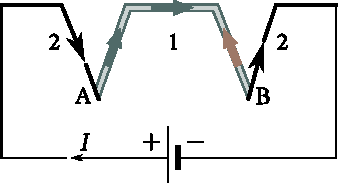
\includegraphics[scale=1]{figures/ch_09/fig_9_3.pdf}
		\caption[]{Diagram of circuit used to observe the Peltier effect.}
		\label{fig:9_3}
	\end{center}
	\vspace{-0.8cm}
\end{figure}

There is a direct connection between the Peltier and Seebeck effects: the temperature difference causes a current to flow in a circuit consisting of different materials and a current flowing through such a circuit sets up a temperature difference. The expression for this relation is due to W. Thomson (Lord Kelvin), who is the author of the thermodynamic theory of thermoelectric phenomena. He demonstrated that:
\begin{equation}\label{eq:9_22}
    \alpha = \frac{\Pi}{T}.
\end{equation}

The Peltier effect is due to the difference in the average energies of the conduction electrons in unlike materials. By way of an example, let's consider the junction of a metal with a nondegenerate n-type semiconductor (\fig{9_4}). After equilibrium had been established their Fermi levels will coincide. Only the electrons close to the Fermi level whose average energy are practically equal to the Fermi energy, take part in the conductivity in the metal.

Denote the average energy of the conduction electrons in the semiconductor by $\ab{\overline{E}}{n}$. This energy is not equal to the thermal energy of the electrons $3\ab{k}{B}T/2$ since the relative part played by fast electrons in the electric current is greater than that of slow electrons. A calculation made for the case of a nondegenerate electron gas yields
\begin{equation}\label{eq:9_23}
    \ab{\overline{E}}{n} = (r+2) \ab{k}{B} T,
\end{equation}

\noindent
where $r$ is the exponent in \eqn{9_13}.

\begin{figure}[t]
	\begin{center}
		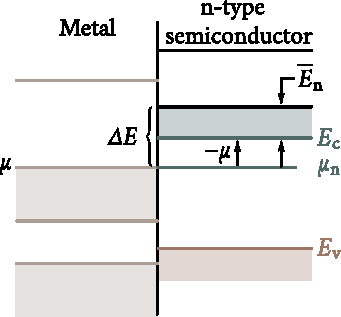
\includegraphics[scale=1]{figures/ch_09/fig_9_4.pdf}
		\caption[]{Energy band pattern of metal-semiconductor junction illustrating mechanism of the Peltier effect.}
		\label{fig:9_4}
	\end{center}
	\vspace{-0.8cm}
\end{figure}

Suppose that the electric current flowing through the junction is such that the electrons flow from the semiconductor to the metal. It may be seen from \fig{9_4}, that each electron that goes over from the semiconductor to the metal carries with it an additional energy equal to
\begin{equation}\label{eq:9_24}
    \Delta{E} = \ab{\overline{E}}{n} + (-\ab{\mu}{n}).
\end{equation}

\noindent
This energy is the Peltier heat and it is liberated near the junction. When the direction of the current is changed, the electrons going over from the metal to the semiconductor absorb heat and cool the junction.

Dividing $\Delta{E}$ by the electron charge, we obtain the Peltier coefficient:
\begin{equation}\label{eq:9_25}
    \ab{\Pi}{mn} = -\frac{\Delta{E}}{q} = -\frac{1}{q} (\ab{\overline{E}}{n} - \ab{\mu}{n}).
\end{equation}

\noindent
Substituting $\ab{\mu}{n})$ from \eqn{3_26} and $\ab{\overline{E}}{n}$ from \eqn{9_23} into \eqref{eq:9_25}, we obtain
\begin{equation}\label{eq:9_26}
    \ab{\Pi}{mn} = - \frac{\ab{k}{B}T}{q} \bracet{  (r+2) + \ln\bracket{ \frac{2 (2 \pi \ab{m}{n} \ab{k}{B} T)^{3/2}}{nh^3} } }.
\end{equation}

A similar relation may be obtained for the junction of a metal with a p-type semiconductor:
\begin{equation}\label{eq:9_27}
    \ab{\Pi}{mp} = - \frac{\ab{k}{B}T}{q} \bracet{  (r+2) + \ln\bracket{ \frac{2 (2 \pi \ab{m}{p} \ab{k}{B} T)^{3/2}}{ph^3} } }.
\end{equation}

For a junction of two metals the Peltier coefficient may be found from \eqn{9_22}:
\vspace{-10pt}
\begin{equation}\label{eq:9_28}
    \Pi_{1,2} = (\alpha_1 - \alpha_2) T.
\end{equation}

\noindent
Substituting $\alpha$ from \eqn{9_12}, we obtain
\begin{equation}\label{eq:9_29}
    \Pi_{1,2} = \frac{\pi^2 \ab{k}{B}^2 T^2}{3q} (1+r) \parenthesis{ \frac{1}{\ab{E}{F$1$}} - \frac{1}{\ab{E}{F$2$}} }.
\end{equation}

\section{The Thomson effect}\label{sec:81}

Imagine a homogeneous conductor AB with a temperature gradient $\diffin{T}{x}$ along its length and carrying a current $I$ [\fig{9_1}(b)]. W. Thomson predicted theoretically that in such a conductor, apart from the Joule heat, an additional amount of heat $Q_{\tau}$ proportional to the current $I$, the temperature difference $(T_2-T_1)$, and the time $t$ should be liberated or absorbed depending on the direction of the current:
\begin{equation}\label{eq:9_30}
    Q_{\tau} = \tau I (T_2 - T_1) t.
\end{equation}

\noindent
The heat $Q_{\tau}$ is termed the \textit{Thomson heat} and the proportionality factor $\tau$ the \textit{Thomson coefficient}. It is determined by the material of the conductor and by temperature. According to Thomson's theory, the difference in Thomson coefficients of two conductors is related to their differential thermoelectric power by the expression:
\begin{equation}\label{eq:9_31}
    \diff{\alpha_{1,2}}{T} = \frac{\tau_1 - \tau_2}{T}.
\end{equation}

The Thomson effect is due to the fact that in a conductor in which a temperature gradient exists, the carrier flux carries not only the electric charge but heat as well. Suppose the current in the conductor AB [\fig{9_1}(b)] flows in the direction corresponding to the electron flow from the hot end B to the cold end A. The ``hot'' electrons as they arrive in the cold regions give up their extra energy and heat the conductor. When the direction of the current is changed, the conductor is cooled.

In quantitative calculations of the Thomson effect one should take into account the thermal emf set up in the conductor, which in the former case will retard the electrons and in the latter accelerate them. This thermal emf can change not only the magnitude of the Thomson coefficient but even its sign.

\section{Galvanomagnetic phenomena}\label{sec:82}

\textbf{The Hall effect.} Suppose a current of density $\vec{i}$ flows in a conducting bar of width $a$ and thickness $b$ (\fig{9_5}). Choose points C and D on the side faces of the bar such that the potential difference between them is zero. Should this bar be placed into a magnetic field with induction $\vec{B}$, potential difference $\ab{V}{H}$ termed \textit{Hall emf} would appear
between points C and D. It follows from experiments that in magnetic fields not too strong
\begin{equation}\label{eq:9_32}
    \ab{V}{H} = \ab{R}{H} B i a.
\end{equation}

\noindent
The proportionality factor $\ab{R}{H}$ is termed the \textit{Hall coefficient}. Its dimensions are L$^3$Q${-1}$ (L is length and Q electric charge) and it is measured in cubic metres per coulomb (\si{\metre\cubed\per\coulomb}). Let us consider the physical origin of the Hall effect.

\begin{figure}[t]
	\begin{center}
		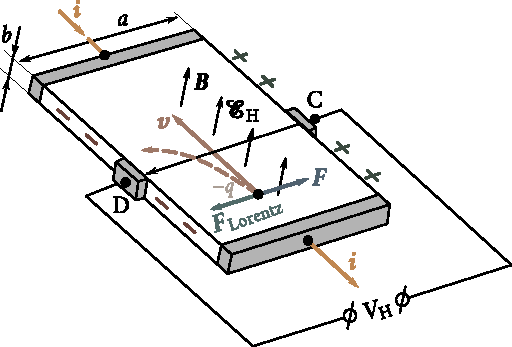
\includegraphics[scale=1]{figures/ch_09/fig_9_5.pdf}
		\caption[]{Layout used to observe the Hall effect.}
		\label{fig:9_5}
	\end{center}
	\vspace{-0.8cm}
\end{figure}

The Lorentz force $\ab{\vec{F}}{Lorentz}$ acting on an electron moving from right to left at a speed $\vec{v}$ (\fig{9_5}) is
\begin{equation*}
    \ab{\vec{F}}{Lorentz} = q \vecprod{v}{B}.
\end{equation*}

\noindent
If $\vec{v}\perp\vec{B}$, the force will be equal to
\begin{equation*}
    \ab{F}{Lorentz} = q v B.
\end{equation*}

The Lorentz force deflects the electrons to the outer face of the bar (dotted line in \fig{9_5}), and the bar receives a negative charge. Uncompensated positive changes accumulate on the opposite side. This results in an electric field directed from C to D:
\begin{equation*}
    \ab{\mathcal{E}}{H} = \frac{\ab{V}{H}}{a},
\end{equation*}

\noindent
where $\ab{V}{H}$ is the potential difference between points C and D (the Hall emf).

The field $\ab{\mathcal{E}}{H}$ exerts a force $F=q\ab{\mathcal{E}}{H}$ on the electrons, this force being directed against the Lorentz force. When $F=\ab{F}{Lorentz}$, the transverse electric field compensates the Lorentz force and no more electric charges are accumulated on the side faces of the bar. From the conditions of equilibrium
\begin{equation}\label{eq:9_33}
    q v B = q \ab{\mathcal{E}}{H},
\end{equation}

\noindent
we obtain
\begin{equation*}
    \ab{\mathcal{E}}{H} = v B.
\end{equation*}

\noindent
Multiplying this relation by the distance $a$ between points C and D, we obtain
\begin{equation*}
    \ab{V}{H} = a \ab{\mathcal{E}}{H} = vBa.
\end{equation*}

\noindent
Taking into account that $i=nqv$ and, consequently $v=i/nq$, we obtain
\begin{equation}\label{eq:9_34}
    \ab{V}{H} = \frac{1}{nq} B i a.
\end{equation}

Thus, theory produces an expression for $\ab{V}{H}$ that coincides with the relation \eqn{9_32} obtained from experiment. The Hall constant turns out to be equal to
\begin{equation}\label{eq:9_35}
    \ab{R}{H} = \frac{1}{nq}.
\end{equation}

\noindent
It follows from \eqn{9_35} that, knowing the absolute value and the sign of the Hall constant, we can find the concentration and sign of the charge carriers in a conductor; $\ab{R}{H}$ of n-type conductors is negative and of p-type conductors positive.

If we measure in addition the specific conductance $\sigma=nqu$ of the conductor, we will be able to find the carrier mobility $u$ since
\begin{equation}\label{eq:9_36}
    \ab{R}{H} \sigma = \ab{u}{H}.
\end{equation}

Mobility $\ab{u}{H}$ determined from \eqn{9_36} is the \textit{Hall mobility} and it may not coincide with the drift mobility defined by \eqn{6_5}.

In the derivation of \eqn{9_35}, it was assumed that all carriers in the conductor have the same speed $v$. Such an assumption is valid in case of metals and degenerate semiconductors but it is totally unacceptable for nondegenerate semiconductors, in which the carrier velocities are distributed in accordance with the Boltzmann law. A more rigorous derivation, which accounts for this fact, yields the following expression for $\ab{R}{H}$:
\begin{equation}\label{eq:9_37}
    \ab{R}{H} = \frac{A}{nq}
\end{equation}

\noindent
where $A$ is a constant dependent on the scattering mechanism of carriers in the crystal. The typical values of $A$ are given in \tab{9_2} below.

In bipolar semiconductors the current is carried simultaneously by electrons and holes. Since their charges are opposite and they move in opposite directions in an electric field, the Lorentz force $\ab{\vec{F}}{Lorentz}=q\vecprod{v}{B}$ deflects them in the same direction. Because of this, other conditions equal, their Hall emf and Hall coefficients will be smaller than in unipolar semiconductors. Calculation yields the following expression for $\ab{R}{H}$ of bipolar semiconductors:
\begin{equation}\label{eq:9_38}
    \ab{R}{H} = \frac{A}{q} \bracket{\frac{\ab{u}{p}^2 p - \ab{u}{n}^2 n}{\parenthesis{\ab{u}{p} + \ab{u}{n}}^2}}
\end{equation}

\noindent
where $n$ and $p$ are electron and hole concentrations, and $\ab{u}{n}$ and $\ab{u}{p}$ their mobilities. Depending on which of the two terms in the numerator is greater, the sign of the Hall coefficient may either be positive, or negative.

For intrinsic semiconductors, in which $n=\ab{n}{i}$, \eqn{9_38} assumes the form:
\begin{equation}\label{eq:9_39}
    \ab{R}{H} = \frac{A}{\ab{n}{i}q} \parenthesis{\frac{\ab{u}{p} - \ab{u}{n}}{\ab{u}{p} + \ab{u}{n}}}.
\end{equation}

\noindent
It follows from \eqn{9_39} that, in the intrinsic range, the sign of the Hall coefficient is determined by that of the carriers with greater mobility. As a rule such carriers are electrons. Therefore, when an extrinsic p-type semiconductor goes over to the intrinsic range, the sign of the Hall coefficients changes. Hall coefficient (at room temperature) for some metals and intrinsic semiconductors is presented below in \tab{9_3}.

As indicated, the Hall coefficient of semiconductors is many
orders of magnitude greater than that of metals. The explanation
is that the carrier concentration in semiconductors is much less
but the mobility, on the other hand, is much greater than in metals.

\bigskip
\bigskip

\begin{table}[h]
	\renewcommand{\arraystretch}{1.2}
	\caption{}
	\vspace{-0.6cm}
	\label{table:9_2}
	\begin{center}\resizebox{0.98\linewidth}{!}{
			\begin{tabular}{lcccc}
				\toprule[1pt]
                 & \multicolumn{3}{c}{\textbf{Scattering on thermal vibrations}} & \multirow{3}{*}{\textbf{Scattering on impurity atoms}}\\
                 \cline{2-4}
                 & \multirow{2}{*}{\textbf{Atomic lattice}} & \multicolumn{2}{c}{\textbf{Ionic lattice}} & \\
                 \cline{3-4}
                 & & $T<\theta$ & $T>\theta$ & \\
                \midrule[0.5pt]\midrule[0.5pt]
                $A$ & $1.17$ & $0.99$ & $1.11$ & $1.93$\\
				\bottomrule[1pt]
			\end{tabular}
	}\end{center}
\end{table}

\begin{table}[h]
	\renewcommand{\arraystretch}{1.2}
	\caption{}
	\vspace{-0.6cm}
	\label{table:9_3}
	\begin{center}\resizebox{0.65\linewidth}{!}{
			\begin{tabular}{lccccc}
				\toprule[1pt]
                 & Cu & Zn & Bi & Ge & Si \\
                \midrule[0.5pt]\midrule[0.5pt]
                $\ab{R}{H}, \parenthesis{\SI{e-11}{\metre\cubed\per\coulomb}}$ & $5.5$ & $3.3$ & \num{e3} & \num{e10} & \num{e13}\\
				\bottomrule[1pt]
			\end{tabular}
	}\end{center}
\end{table}

\textbf{Ettingshausen effect.} The thermal velocities of electrons in nondegenerate semiconductors lie in a wide range. In such conditions, \eqn{9_33} may be valid not for all the electrons but only for some of them whose average velocity is $v_0$. For electrons whose velocity is $v>v_0$, we have $qvB>q\ab{\mathcal{E}}{H}$ and they will be deflected to the right-hand face of the plate [\fig{9_6}(a)]. The electrons whose velocity is $v<v_0$, so that $qvB<q\ab{\mathcal{E}}{H}$, will be deflected to the left-hand face of the plate.

Fast electrons reaching the right-hand face give up their extra energy to it and thereby heat it. The slow electrons, which accumulate on the left-hand face, replenish their energy deficit at the expense of the thermal energy of the crystal and thereby cool it. Thus, a transverse temperature difference $T=\ab{T}{D}-\ab{T}{C}$ is established. This phenomenon is termed \textit{Ettingshausen effect}.

\begin{figure}[t]
	\begin{center}
		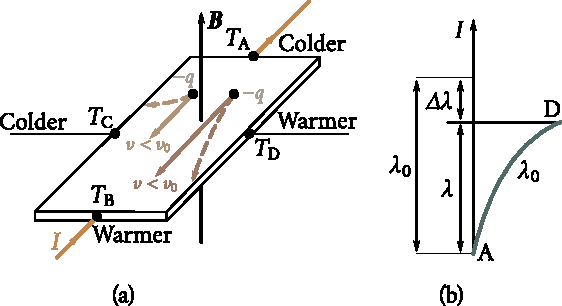
\includegraphics[scale=1]{figures/ch_09/fig_9_6.pdf}
		\caption[]{Diagram explaining the origin of the Ettingshausen and Nernst effects (a) and of specific resistance variations in magnetic field (b).}
		\label{fig:9_6}
	\end{center}
	\vspace{-0.8cm}
\end{figure}

\textbf{Nernst effect.} The electrons entering a homogeneous magnetic field $B$ perpendicular to their velocity $v$ start moving in a circle with a radius
\begin{equation}\label{eq:9_40}
    r = \frac{\ab{m}{n} v}{q B}.
\end{equation}

\noindent
It follows from \eqn{9_40} that the fast electrons are rotated by the magnetic field less than the slow electrons [\fig{9_6}(a)]. Therefore, the front face of the plate will be richer in hot electrons and will be heated while the back face will be richer in slow electrons and will be cooled. A longitudinal temperature difference $\ab{T}{B}-\ab{T}{A}$ will be established. This is the \textit{Nernst effect}.

\textbf{Variation of conductor's resistance in magnetic fields (magnetoresistance).} The trajectories of electrons moving in a magnetic field with velocities other than $v_0$ are curved [\fig{9_6}(a)] and this results in a reduction of their effective mean free path in the direction of the electric current. If the mean free path in the direction of the current in the absence of a magnetic field is $\lambda_0$, in the magnetic field it is equal to the projection of the arc AD on the direction of the current $I$, that is $\lambda=\lambda_0-\Delta{\lambda}$ [\fig{9_6}(b)].

Since the carrier mobility $u$ is proportional to the mean free path, the decrease in the mean free path by $\Delta{\lambda}$ should bring about a decrease in mobility by $\Delta{u}$ and in the semiconductor's conductivity by $\Delta{\sigma}$, so that
\begin{equation*}
    \frac{\Delta{\sigma}}{\sigma} = \frac{\Delta{u}}{u} = \frac{\Delta{\lambda}}{\lambda_0}.
\end{equation*}

The theory provides the following expression for the relative increase in specific resistance of extrinsic unipolar semiconductors:
\begin{equation}\label{eq:9_41}
    \frac{\Delta{\rho}}{\rho} = c u^2 B^2,
\end{equation}

\noindent
where $B$ is the magnetic field induction, and $c$ a coefficient dependent on the carrier scattering mechanism.

The ratio $\Delta{\rho}/\rho$ is termed \textit{magnetoresistivity}. It follows from \eqn{9_41} that, by measuring magnetoresistivity, one can directly find the carrier mobility.

\section{Practical applications of thermoelectric
and galvanomagnetic phenomena}\label{sec:83}

\textbf{Thermoelectric phenomena.} For a long time the only application of the Seebeck effect was in measurements. Placing one junction of a thermocouple in a thermostat, held at a known constant temperature
and the other junction into the object the temperature of which is to be measured, one can determine this temperature from the thermal emf established in the couple. Such measurements are quite simple, reliable and sufficiently accurate and can be carried out in a wide temperature range.

However, after semiconductors were discovered it became possible to use the Seebeck effect for the direct conversion of thermal energy into electric energy. The devices used to this end are termed thermoelectric generators and the elements of which they are assembled thermoelements. The man mainly responsible for their development and wide publicity was the Soviet physicist A. F. Ioffe.

The first thermoelectric generators were produced before World War II and were used in the war to power radio equipment. The thermoelectric generators were mounted in the bottom of a special kettle and heated in the process of boiling water.

In 1953 a commercial type of thermoelectric generator of \SI{3}{\watt} power for battery receivers was produced; later thermoelectric generators of \SI{1}{\kilo\watt} power and more were produced. Presently generators designed for hundreds of kilowatts are being developed.

The midseventies saw the appearance of thermoelectric generators utilizing the heat of radioactive decay of chemical elements. An example of such a generator is the generator Beta-$1$ with a power of \SIrange{150}{200}{\watt}, which operates on the radioactive cerium isotope Ce-$144$. It was designed to power electronic equipment of automatic radiometeorologic stations, earth satellites, etc.

In 1964 an experimental atomic reactor-energy converter Romashka (Camomile) with a power of \SI{500}{\watt} for direct conversion of heat energy into electric energy was built.

Work is in progress on thermoelectric generators that would utilize the thermal energy of the sun's radiation.

It is a regretful fact, but the efficiency of even the best modern experimental thermoelements does not rise above $8\%$.

The Peltier effect is beginning to be widely used in practice mainly for various cooling devices: home refrigerators, devices for cooling aircraft electronic equipment, microcoolers for biological applications, various thermoelectric thermostats, temperature-controlled microscope supports, etc. Quite possible, the Peltier effect will in the near future be used for heating dwellings in winter and for cooling them in summer.

\textbf{Galvanomagnetic phenomena.} The most widely used galvanomagnetic phenomenon is the Hall effect. Apart from applications in the study of electric properties of materials it served as a basis for the design of a wide class of instruments: magnetometers, dc-ac and ac-dc converters, signal generators, phase meters, microphones, etc.

In recent years attempts are made to use the Ettingshausen effect in cooling devices. With the right choice of materials and with the optimal geometry of the cooling crystal it is possible to obtain temperatures of the cold face of the crystal of over \SI{100}{\degreeCelsius} below that of the surroundings.


% \begin{figure}[!t]
% 	\begin{minipage}[t]{0.48\linewidth}
% 		\begin{center}
%             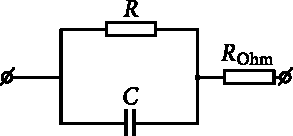
\includegraphics[scale=0.98]{figures/ch_08/fig_8_19.pdf}
%             \caption[]{Equivalent circuit of diode: $R$---non-linear resistance of p-n junction, $C$---capacitance of p-n junction; $\ab{R}{ohm}$---ohmic resistance of passive regions and contacts.}
%             \label{fig:8_19}
% 		\end{center}
% 	\end{minipage}
% 	\hfill{ }%\hspace{-0.1cm}
% 	\begin{minipage}[t]{0.48\linewidth}
% 		\begin{center}
% 			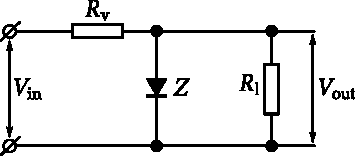
\includegraphics[scale=0.98]{figures/ch_08/fig_8_20.pdf}
% 			\caption[]{Circuit diagram of the simplest voltage regulator using a silicon Zener diode $Z$.}
% 			\label{fig:8_20}
% 		\end{center}
% 	\end{minipage}
% \vspace{-0.3cm}
% \end{figure}
